\section{Segurança, Privacidade e Legislação}
Atualmente, há uma crescente no número de usuários utilizando dispositivos conectados a \textit{Internet}, o que, por um lado mostra que essa tecnologia tão importante está sendo difundida a todas as camadas sociais, mas por outro, gera preocupação quanto as implicações do uso inadvertido das redes.
Nesse contexto, tornou-se comum pessoas mal intencionadas que usam da ignorância de alguns para cometer ataques digitais, prejudicando ou tomando vantagem de pessoas, grupos ou organizações. A afirmativa anterior é confirmada por um gráfico (Figura \ref{fig:cibercrimes}) elaborado pela Surfshark \cite{Surfshark}, empresa provedora de serviços de VPN, que analisa o crescimento anual de custos em cibersegurança. 
\begin{figure}[h]
	\centering
	\caption{Crescimento anual de custos com cibercrime}
	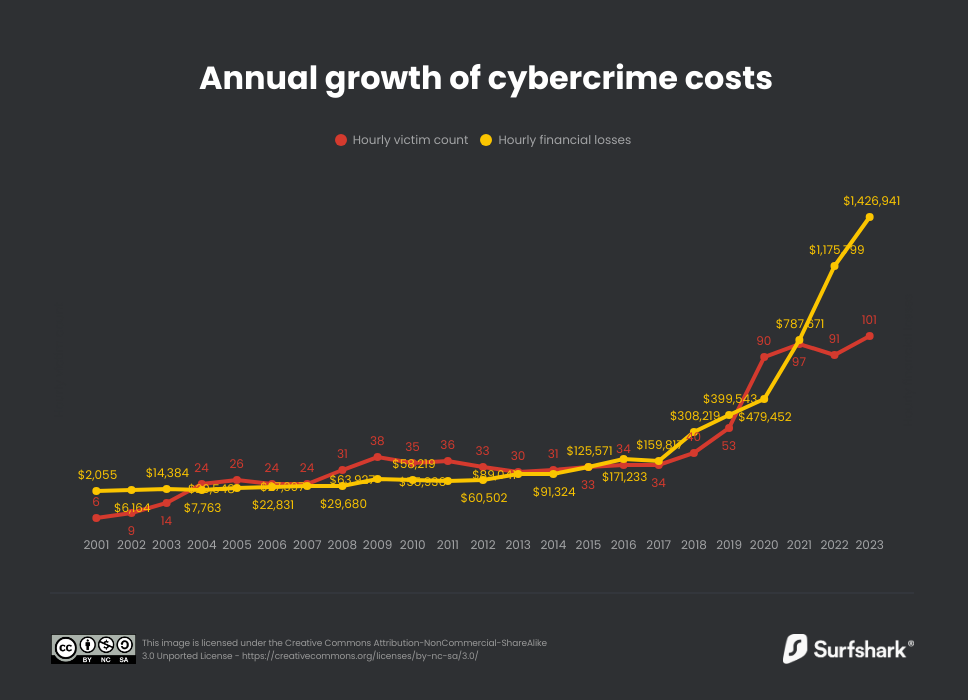
\includegraphics[width=1\textwidth]{cap04-desenvolvimento/images/4-6-annual-growth-of-cybercrime-costs.png}
	\fonte{Surfshark}
	\label{fig:cibercrimes}
\end{figure}

Por isso surgiram leis e normas que regularizam como os dados devem ser tratados e também tecnologias que auxiliam a proteger os dois lados da comunicação: os clientes, que desejam ter seus dados protegidos, e das organizações, que precisam se certificar da identidade do usuário.
Isto posto, serão abordadas as técnicas e metodologias adotadas a fim de garantir que o software desenvolvido atenda as demandas da legislação e promova segurança e privacidade a seus utilizadores.

\subsection{Critérios de segurança e privacidade}
Na aplicação desenvolvida, foram definidas formas de manter a segurança de todas as partes envolvidas. Foi implementado um método de cadastro e \textit{login} facilitado com geração de \textit{tokens} e também uma infraestrutura de rede que protege o dispositivo que armazena o banco de dados da aplicação.

\subsubsection{Cadastro e login com conta Google}
Um dos requisitos da entidade parceira, era o desenvolvimento de um sistema de cadastro e login facilitados, haja vista que muitos dos clientes tinham dificuldade em acessar a aplicação anterior por constantemente esquecerem sua credenciais (e-mail e senha).
Considerando essa dificuldade, foi implementado um sistema de registro e login utilizando a API de autenticação OAuth da Google, pelo fato da maioria dos dispositivos no Brasil apresentarem sistema operacional Android, conforme destaca uma pesquisa \cite{app-my-site}, que geralmente requerem uma conta Google para seu funcionamento. E mesmo indivíduos com aparelhos de outro sistema operacional, comumente possuem contas Google para usufruir de seus serviços.
Assim sendo, a responsabilidade de identificar os usuários da aplicação foi terceirizada para a Google, e quando estes se cadastram, devem aceitar sua políticas e termos de usuário que definem extensamente como os dados são processados, tratados e protegidos.

\subsubsection{Infraestrutura de Rede}
Os dispositivos (máquinas virtuais) que sustentam a aplicação estão hospedados na AWS, logo sendo de sua inteira responsabilidade protegê-los fisicamente, como diz seu Modelo de Responsabilidade Compartilhada \cite{aws-shared-responsibilities}, porém no que tange a software e redes, cabe ao time de desenvolvimento proteger.
Para evitar acessos indevidos aos sistema interno, criaram-se duas instâncias EC2, uma delas sendo pública e outra privada. Como já explicado, a instância privada não possui IP público, portanto só é possível acessá-la pela rede interna dentro da infraestrutura de rede criada, delimitando uma camada a mais de segurança.
O acesso a essa instância é feito pela instância pública por meio do protocolo SSH, que possui seus próprios métodos de segurança com esquema de chaves de acesso.
\subsection{Observância à Legislação}